\documentclass{beamer}

\usepackage{amsmath, amssymb}

\title{Carr-Madan Spanning Formula \& VIX}
\subtitle{Math 490 - Research Project}
\author{Artem Ivaniuk, Andy Chang, Krishaan Chaudhary}
\date{\today}

\begin{document}

\frame{\titlepage}

%------------------------------------------------

\begin{frame}{Carr-Madan: Idea}
Goal: replicate nonlinear option payoff with a portfolio of options

\[
g(S_t)
=
\]
\[
g(F) + g'(F)(S_t - F)
+ \int_0^F g''(K)(K - S_t)^+ dK
+ \int_F^\infty g''(K)(S_t - K)^+ dK
\]

\begin{itemize}
\item $g(S_t)$ = value of derivative
\item $F$ is a constant
\item European style payoff - payoff at expiration
\item Enables a static hedge of complex options using puts and calls

\end{itemize}
\end{frame}

%------------------------------------------------

\begin{frame}{Carr-Madan: Derivation Intuition}
\[
g(x) = g(a) + \int_a^x g'(t) dt
\]
\[
g(x) = g(a) + \int_a^x [g'(t) + g'(a) - g'(a)] dt
\]
\[
g(x) = g(a) + g'(a)(x-a) +\int_a^x [g'(t)-g'(a)] dt 
\]
\[
g(x) = g(a) + g'(a)(x-a) + \int_a^x \left[ \int_{u=a}^{u=t}g''(u) du \right] dt
\]
\[
g(x) = g(a) + g'(a)(x-a) + \int_a^x \left[ \int_{t=u}^{t=x}g''(t) dt \right]du
\]
\[
g(x) = g(a) + g'(a)(x-a) + \int_a^x g''(u) (x-u) du
\]

\begin{itemize}
\item FTC, Adding Zero, Integrate constant, Rewrite as Double Integral, Fubini's Theorem

\end{itemize}
\end{frame}

%------------------------------------------------

\begin{frame}{Carr-Madan: Derivation Intuition}
\[
H(x) =
\begin{cases}
0 & \text{if } x < 0 \\
1 & \text{if } x \ge 0
\end{cases} \quad \quad H(x) + H(-x) = 1
\]
\[
\int_a^x g''(u) (x-u) du = \int_a^x [H(x-a) + H(a-x)]g''(u) (x-u) du
\]
\[
= \int_a^x H(x-a)g''(u) (x-u) du + \int_x^a H(a-x)g''(u) (u-x) du
\]
\[
\dots  = \int_a^\infty (x-u)^+ g''(u) du + \int_{-\infty}^a (u-x)^+g''(u)du
\]


\begin{itemize}
\item Heaviside Function, Symmetry, Extending Bounds, Piecewise Function Properties

\end{itemize}
\end{frame}

%------------------------------------------------

\begin{frame}{VIX as a Target}
VIX measures:
\[
\frac{1}{T}\mathbb{E}\left[\int_0^T \sigma_t^2 dt\right]
\]

Interpretation:
\begin{itemize}
\item Risk-neutral expected variance
\item Derived from S\&P500 options across past 30 days' strikes
\item Option prices encode volatility
\item Described as a "fear gauge"
\item Although not directly traded, there are futures and ETFs
\item Can develop a replicating portfolio to hedge against uncertainty
\item Can be used in trading strategies for insurance against downturn or a way to trade volatility itself

\end{itemize}


\end{frame}

%------------------------------------------------

\begin{frame}{VIX During 2008 Financial Crisis}
\begin{figure}
    \centering
    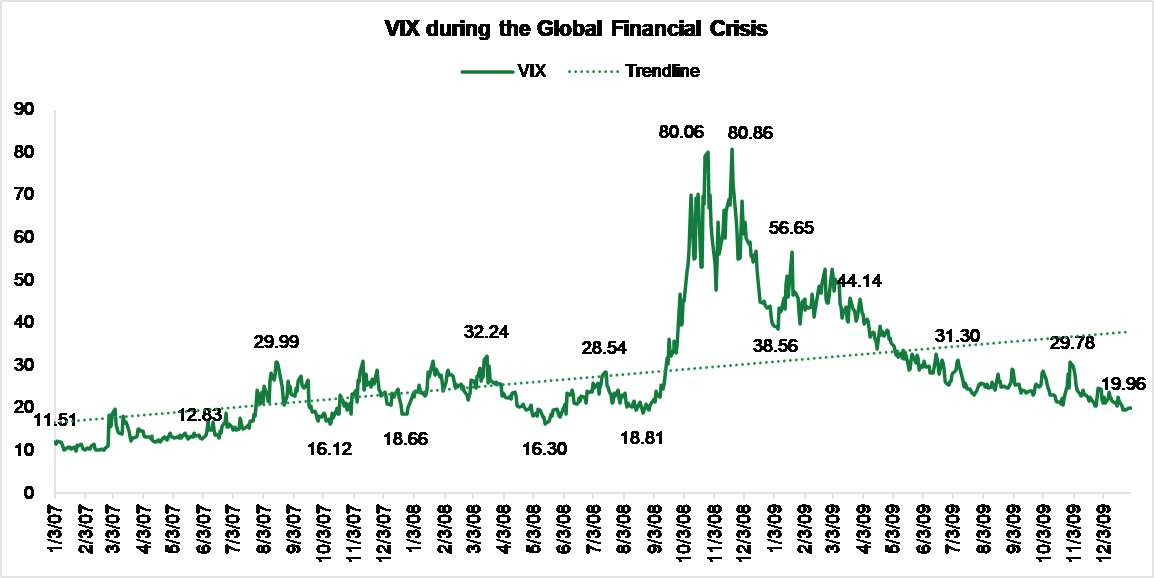
\includegraphics[width=1\linewidth]{image.png}
\end{figure}
\end{frame}

%------------------------------------------------

\begin{frame}{VIX Formula}

\[
\text{VIX}^2
\approx \frac{2}{T} \sum_i \frac{\Delta K_i}{K_i^2} Q(K_i)
\]

\begin{itemize}
\item $Q(K_i)$: OTM (Out of the Money) option prices
\item OTM options encapsulate market sentiment about extreme changes
\item puts for $K_i < F$, calls for $K_i > F$
\item $\Delta K_i$: strike spacing
\item $\frac{2}{T}$: scaling factor for time
\item $\frac{1}{K_i^2}$: lower strike prices weighted more

\end{itemize}
\end{frame}

%------------------------------------------------

\begin{frame}{Log Dynamics $\rightarrow$ Expected Variance}
\[
d\log S_t = \left(r - \frac{1}{2}\sigma_t^2\right) dt + \sigma_t dW_t
\]
\[
\log S_T - \log S_0
= \int_0^T \left(r - \frac{1}{2}\sigma_t^2\right) dt
+ \int_0^T \sigma_t dW_t
\]
\[
\mathbb{E}[\log S_T]
= \log S_0 + rT - \frac{1}{2}\mathbb{E}\left[\int_0^T \sigma_t^2 dt\right]
\]
\[
\mathbb{E}\left[\int_0^T \sigma_t^2 dt\right]
= -2\,\mathbb{E}\left[\log\left(\frac{S_T}{F}\right)\right]
\]

\begin{itemize}
\item Ito's Lemma converts price dynamics into log form with variance appearing explicitly $\rightarrow$ we now can isolate variance
\item Stochastic integral drops out under expectation (martingale)
\item Isolating integrated variance as a function of log-returns
\item Forward price $F = S_0 e^{rT}$ simplifies expectation
\end{itemize}
\end{frame}

%------------------------------------------------

\begin{frame}{Eliminating Linear Terms $\rightarrow$ Pricing Identity}
\[
f(S_T) = -2 \log\left(\frac{S_T}{F}\right), \quad f''(K) = \frac{2}{K^2}
\]
\[
f(F) + f'(F)(S_T - F) = -\frac{2}{F}(S_T - F)
\]
\[
\mathbb{E}[S_T] = F \Rightarrow \text{term vanishes}
\]
\[
\mathbb{E}[f(S_T)]
=
\int_0^F \frac{2}{K^2} P(K)\, dK
+ \int_F^\infty \frac{2}{K^2} C(K)\, dK
\]
\[
\mathbb{E}[f(S_T)] = \mathbb{E}\left[\int_0^T \sigma_t^2 dt\right]
\]

\begin{itemize}
\item Linear terms cancel under risk-neutral expectation
\item Remaining terms are purely option payoffs 
\item Put and call prices replace expectations of $(\cdot)^+$ payoffs
\item We got a link between option prices and expected variance
\end{itemize}
\end{frame}

%------------------------------------------------

\begin{frame}{From Integral to VIX Formula: Intuition}
\[
\mathbb{E}\left[\int_0^T \sigma_t^2 dt\right]
=
\int_0^\infty \frac{2}{K^2} Q(K)\, dK
\]
\[
\int_0^\infty \frac{2}{K^2} Q(K)\, dK
\approx
\sum_i \frac{2}{K_i^2} Q(K_i)\, \Delta K_i
\]
\[
\text{VIX}^2 \approx \frac{2}{T} \sum_i \frac{\Delta K_i}{K_i^2} Q(K_i)
\]

\begin{itemize}
\item Combine puts and calls into unified OTM price function $Q(K)$
\item Extend integration over all strikes using payoff symmetry
\item Replace integral with discrete sum over traded strikes
\item Normalize by maturity $T$ to obtain implied variance (VIX)
\end{itemize}
\end{frame}

%------------------------------------------------

\begin{frame}{Numerical Approximation}

For the numerical approximation, we used \textbf{yfinance}, a Python api for Yahoo Finance ticker information. \\

Key points about our approach: 
\begin{itemize}
    \item We used S\&P500 index put / call prices to price VIX 
    \item SPX index offers European Options, one of the assumptions needed for the Carr-Madan spanning formula  
    \item We consider the midpoint of the bid / ask prices on an option to be its price. 
\end{itemize}

\end{frame}

%------------------------------------------------

\begin{frame}{Numerical Approximation Inputs / Output}

Inputs: 

\begin{itemize}
\item Current Date
\item S\&P500 Current Price
\end{itemize}

Run Conditions:
\begin{itemize}
\item $r=4.31\%$ (annual interest rate)
\item Timestamp of run: 04-25-2026 9:58pm
\end{itemize}

Output is the approximated VIX price 

\end{frame}

%------------------------------------------------

\begin{frame}{Results + Comparison}

\begin{figure}
    \centering
    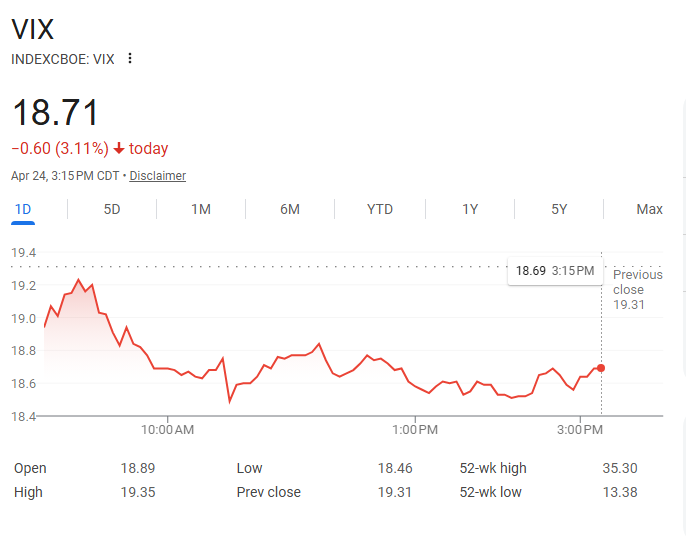
\includegraphics[width=0.5\linewidth]{vix.png}
    \caption{Vix price at close on 04-24-26}
    \label{fig:vix}
\end{figure}

Code output results:

\texttt{Option Expiry Date: 2026-05-26 \\ 
S0: 7165.08 \\ 
Sigma squared term: 0.03508 \\ 
VIX via Carr-Madan: 18.7309 }

\end{frame}

%------------------------------------------------

\begin{frame}{Ta-Dah!}
Thank you!

Any questions?
\end{frame}

\end{document}